%%
%  ******************************************************************************
%  * #file    Szablon_raportu_EN_Latex.tex
%  * #author  Adrian Wójcik   adrian.wojcik(at)put.poznan.pl
%  *          
%  * #commit  Patryk Kościk   koscikpatryk(at)gmail.com
%  *          Modified the template for Projekt przejsciowy purposes          
%  *          
%  *
%  * #commit  Patryk Kościk   koscikpatryk(at)gmail.com
%  *          Zupełnie przewrócono na łeb formatke po taktycznym wyjasnieniu          
%  *          
%  * #version 1.1
%  * #date    09-Mar-2022
%  * #brief   PROJPRZEJ
%  *
%  ******************************************************************************
%%  
\documentclass[11pt, a4paper]{article}

\usepackage{SM_template}

% Wypełnijcie te dyrektywy zgodnie z waszym tematem
%
% \lab      -> NAZWA CZUJNIKA,          np.: 'DHT22'
% \comment  -> Króciutki opis co to,    np.: 'Cyfrowy czujnik temperatury'
% \author   -> Autor dokumentu          np.: Patryk Kościk
%
% Pamiętajcie o zmianie ścieżki w \addbibresourcue (!)

\lab{Moduł KY-039}
\comment{Analogowy czujnik tętna}
\author{Anna Nasierowska}
\addbibresource{bib/KY-039.bib}
\nocite{*}

%
% Początek dokumentu
%
\begin{document}
%% Strona tytułowa %%
\mainpage{{KY-039/tytulowy}}
\newpage

\section*{Opis elementu} \addcontentsline{toc}{section}{Wstęp}

Sensor w tym module to \textbf{fototranzystor} działający w zakresie podczerwieni. Jest to analogowy czujnik, którego napięcie kolektor-emiter jest wyjściem z modułu. Odbiera on fale nadawane przez diodę IR, które przedostają się przez palec. \\

\vspace{0.5cm}
\begin{figure}[h]
\centering
\begin{subfigure}{.5\textwidth}
  \centering
  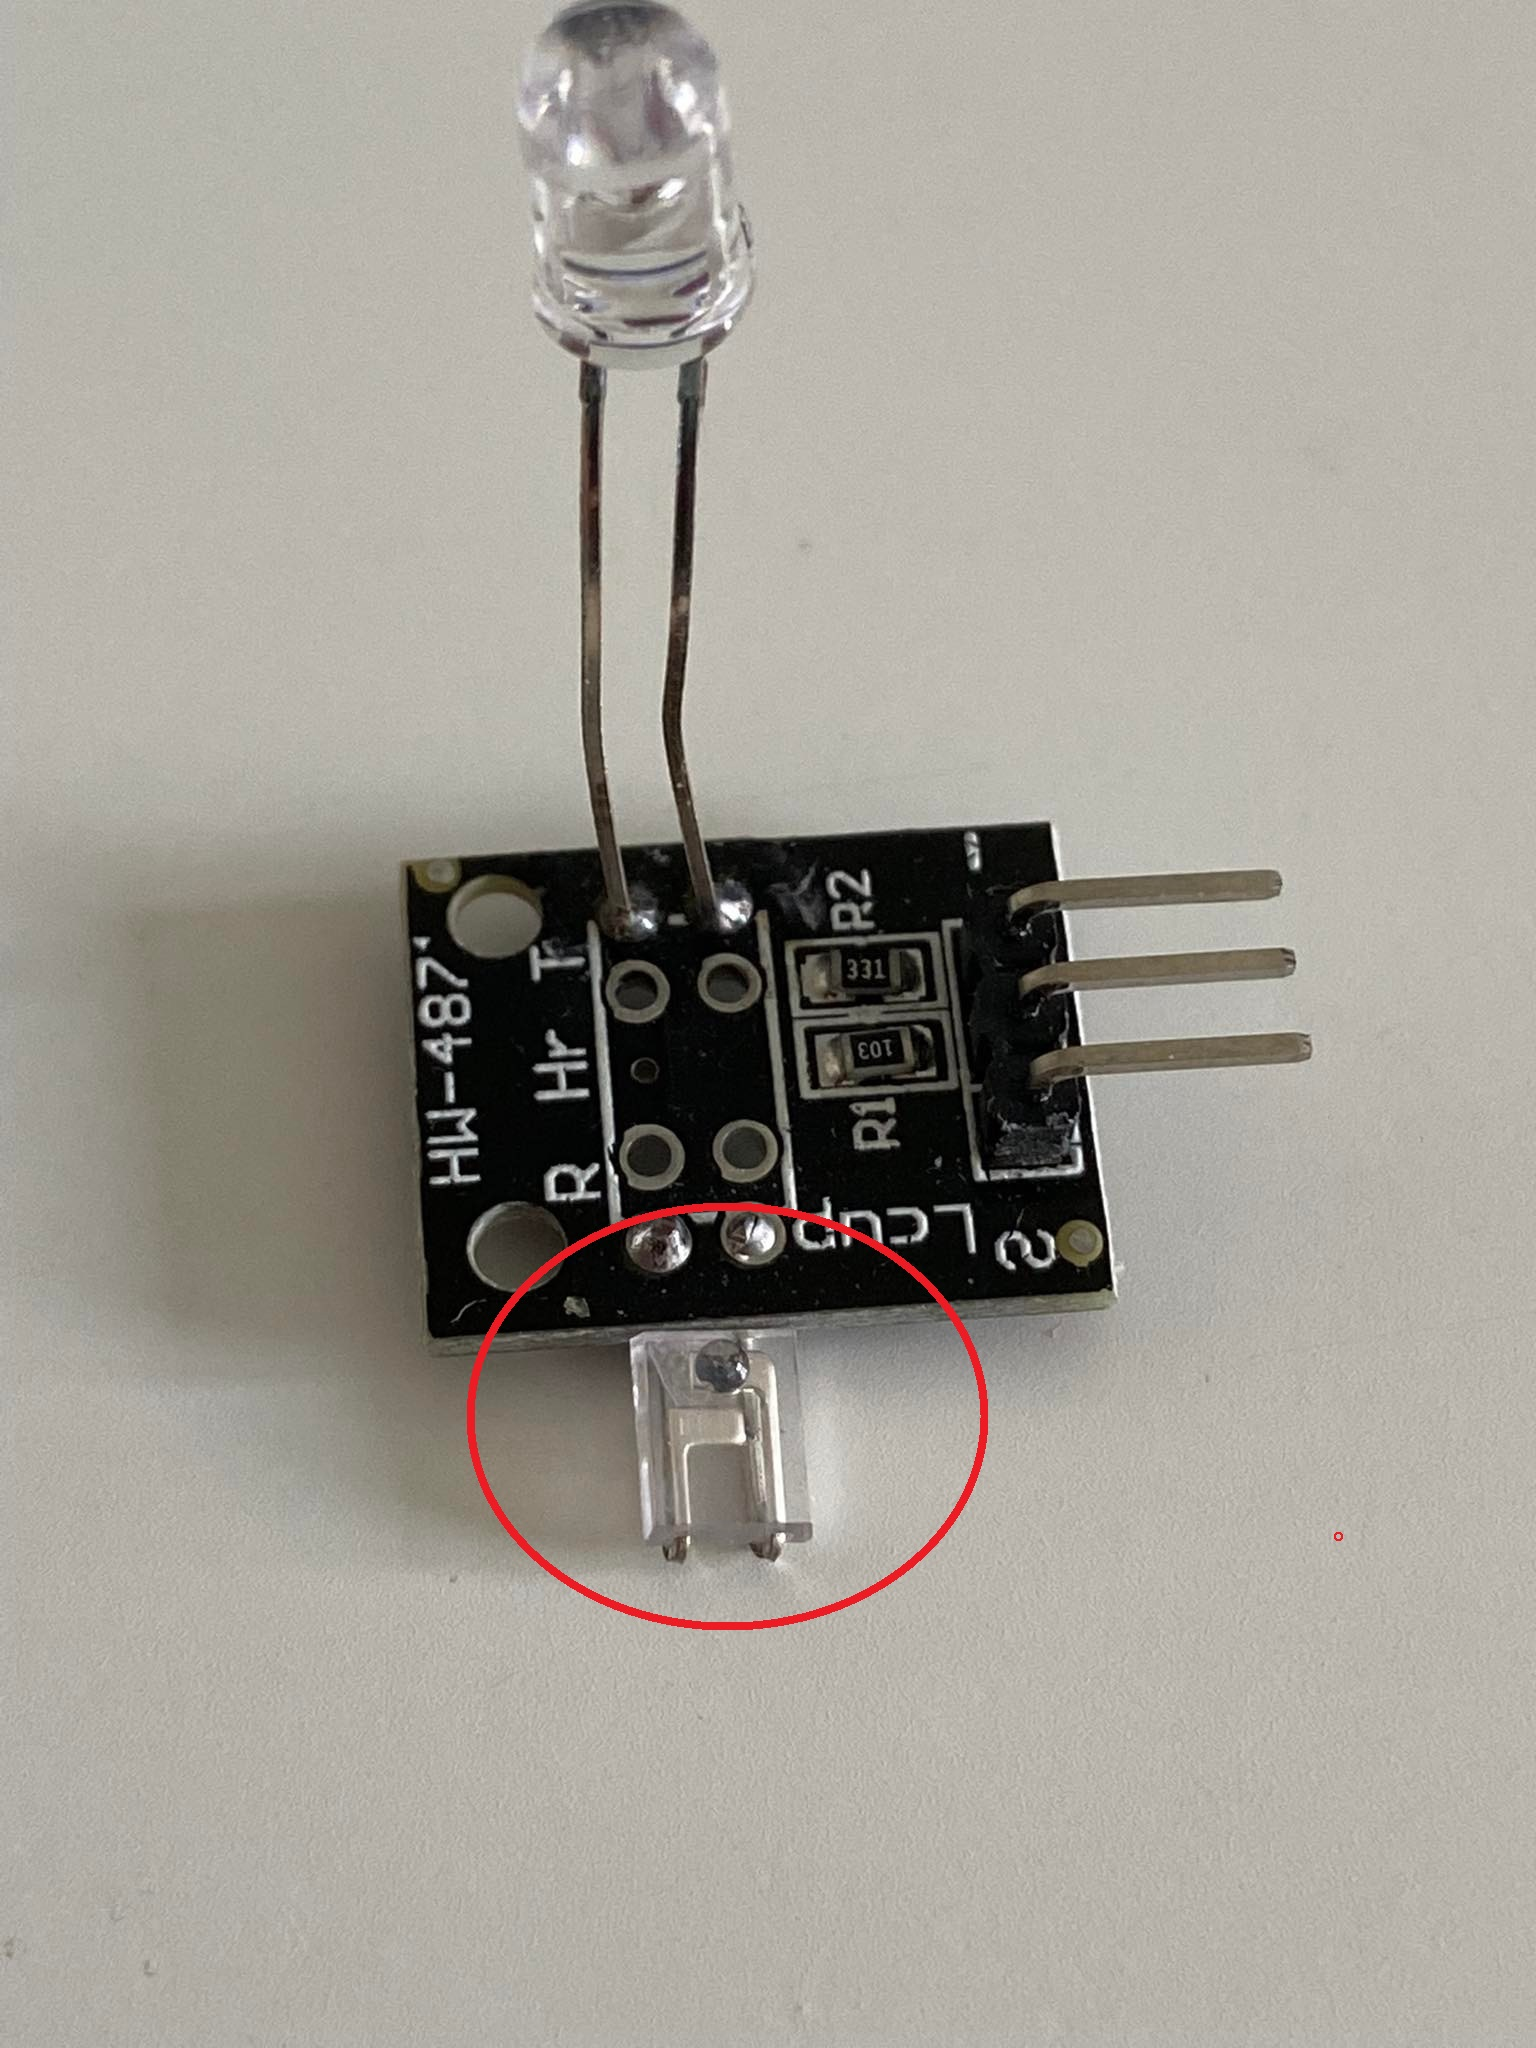
\includegraphics[width=.5\linewidth]{fig/KY-039/zdj_modułu/zdj1.jpg}
  \caption{Zdjęcie odbiornika w module}
  \label{fig:sub1}
\end{subfigure}%
\begin{subfigure}{.5\textwidth}
  \centering
    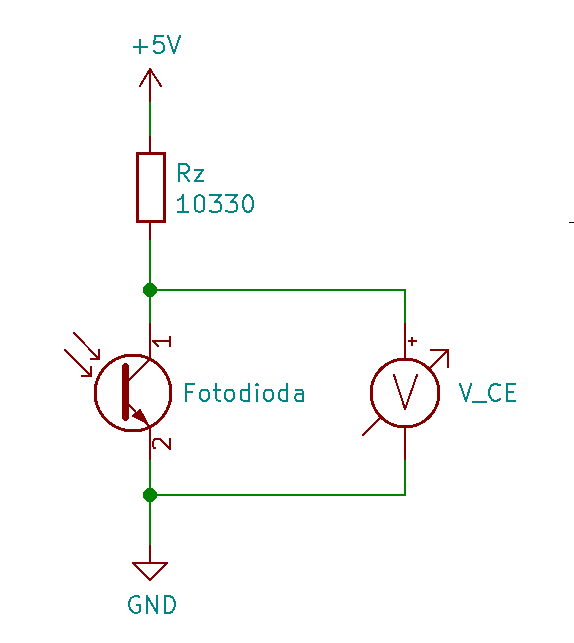
\includegraphics[width=.6\textwidth]{fig/KY-039/zasada_dzialania/odbiornik_sch.png}
      \caption{Schemat ideowy sensora w układzie}
  \label{zd}
\end{subfigure}
\caption{Czujnik}
\label{fig:test}
\end{figure}
\vspace{0.5cm}

Omawiany moduł składająca się z 3 pinów - masa, +5V lub +3.3V oraz AO (Analog Output), 2 wbudowanych rezystorów, y świecącej w podczerwieni oraz wystającego za płytkę odbiornika IR. Służy on do pomiaru tętna przez palec, poprzez położenie go pomiędzy diodą a fototranzystorem. Naczynia krwionośne w ludzkim ciele regularnie poszerzają się i zwężają w rytmie bicia serca, blokując więcej lub mniej podczerwonego światła przechodzącego przez palec. Czujnik podaje na pin wyjściowy analogowy napięcie o wartości 0-5V, gdzie większa wartość oznacza, że w danym momencie mniej podczerwonego światła dostało się na odbiornik. 

\vspace{0.5cm}
\begin{figure}[h]
\centering
\begin{subfigure}{.4\textwidth}
  \centering
  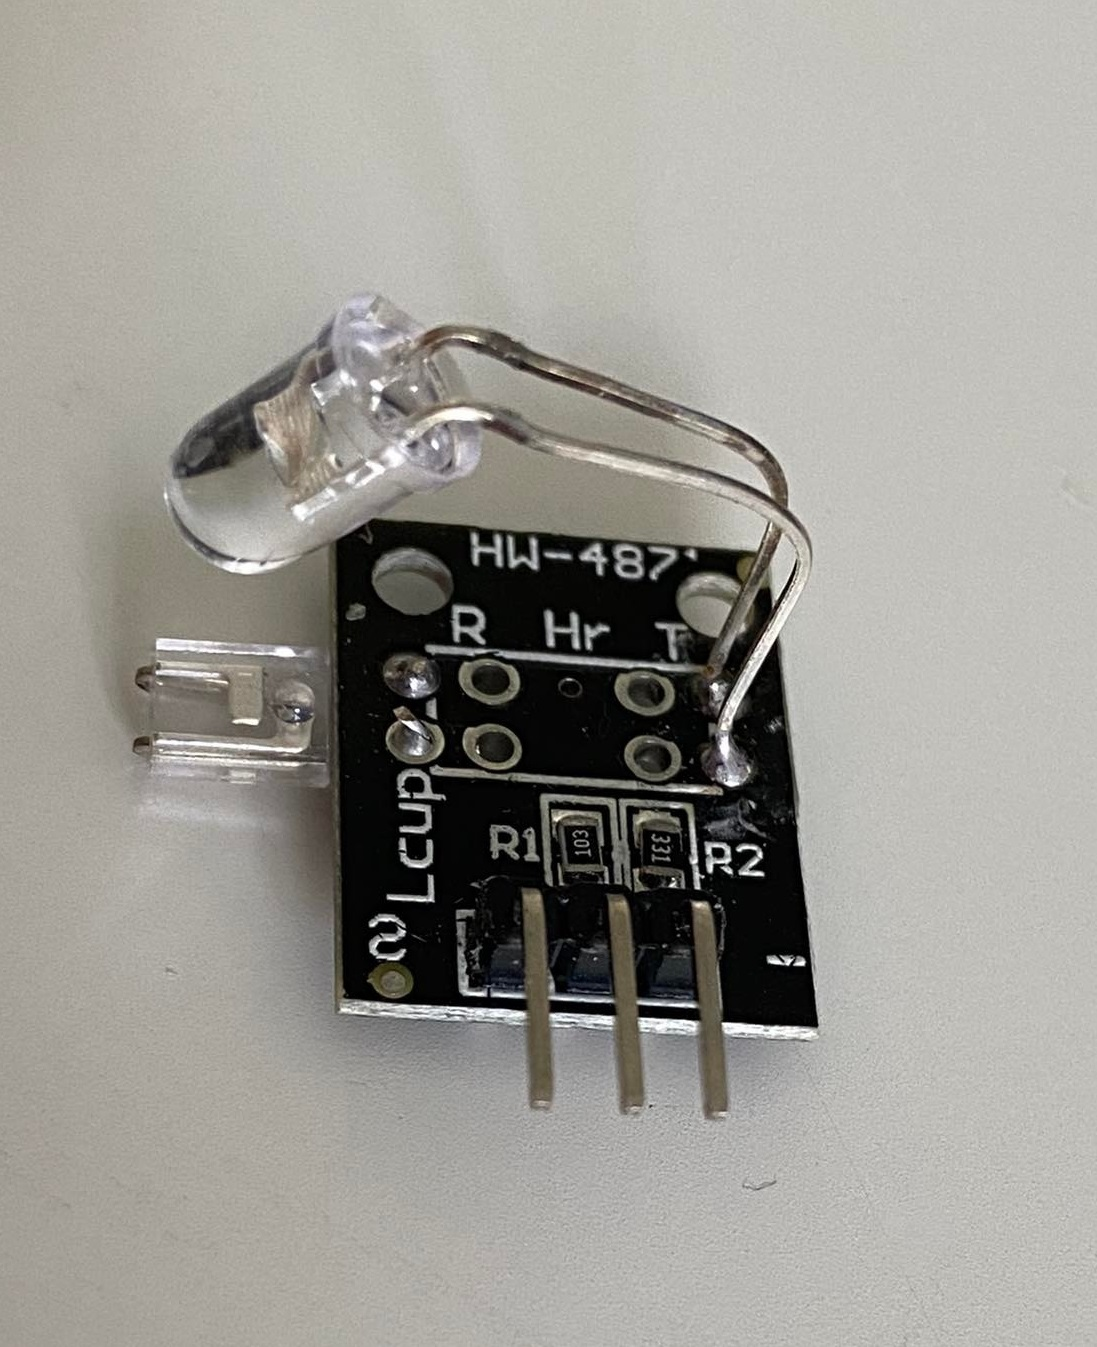
\includegraphics[width=.4\linewidth]{fig/KY-039/zdj_modułu/zdj2.jpg}
  \caption{Zdjęcie modułu}
  \label{fig:sub1}
\end{subfigure}%
\begin{subfigure}{.4\textwidth}
  \centering
    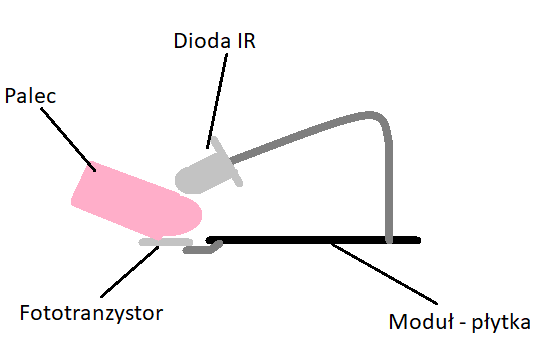
\includegraphics[width=.8\textwidth]{fig/KY-039/zasada_dzialania/rysunek.png}
      \caption{Zasada działania}
  \label{zd}
\end{subfigure}
\caption{Moduł}
\label{fig:test}
\end{figure}
\vspace{0.5cm}
Na zasadzie analogicznej do działania omawianego modułu wykonane są np. czujniki tętna w sportowych zegarkach. 


\vspace{0.5cm}
\begin{figure}[h]
  \centering
  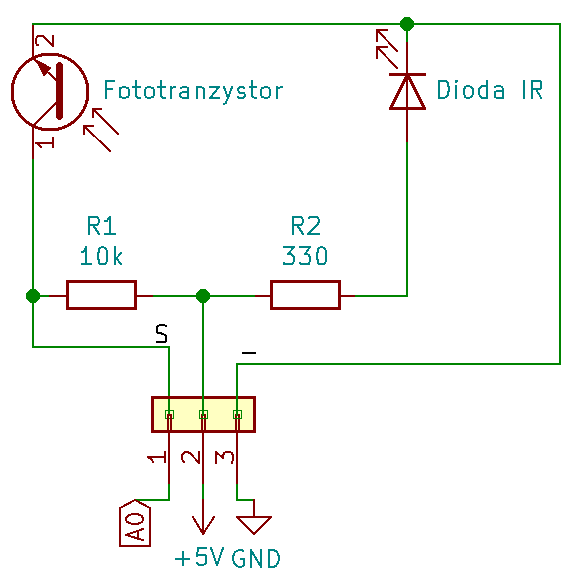
\includegraphics[width=.5\textwidth]{fig/KY-039/polaczenie_modulu/modul_sch.png}
    \caption{Schemat modułu}
    \label{sch}
\end{figure}


\section{Użycie czujnika}
W celu prezentacji użycia czujnika podłączono go do napięcia +5V oraz miernika. Można zaobserwować, że gdy światło pada bezpośrednio na fototranzystor, napięcie na wyjściu modułu jest bliskie zera. Natomiast, gdy na drodze pojawia się palec znacznie mniej światła dociera i amplituda sygnału prawie dochodzi do wartości maksymalnej. 

\vspace{0.5cm}
\begin{figure}[h]
\centering
\begin{subfigure}{.5\textwidth}
  \centering
  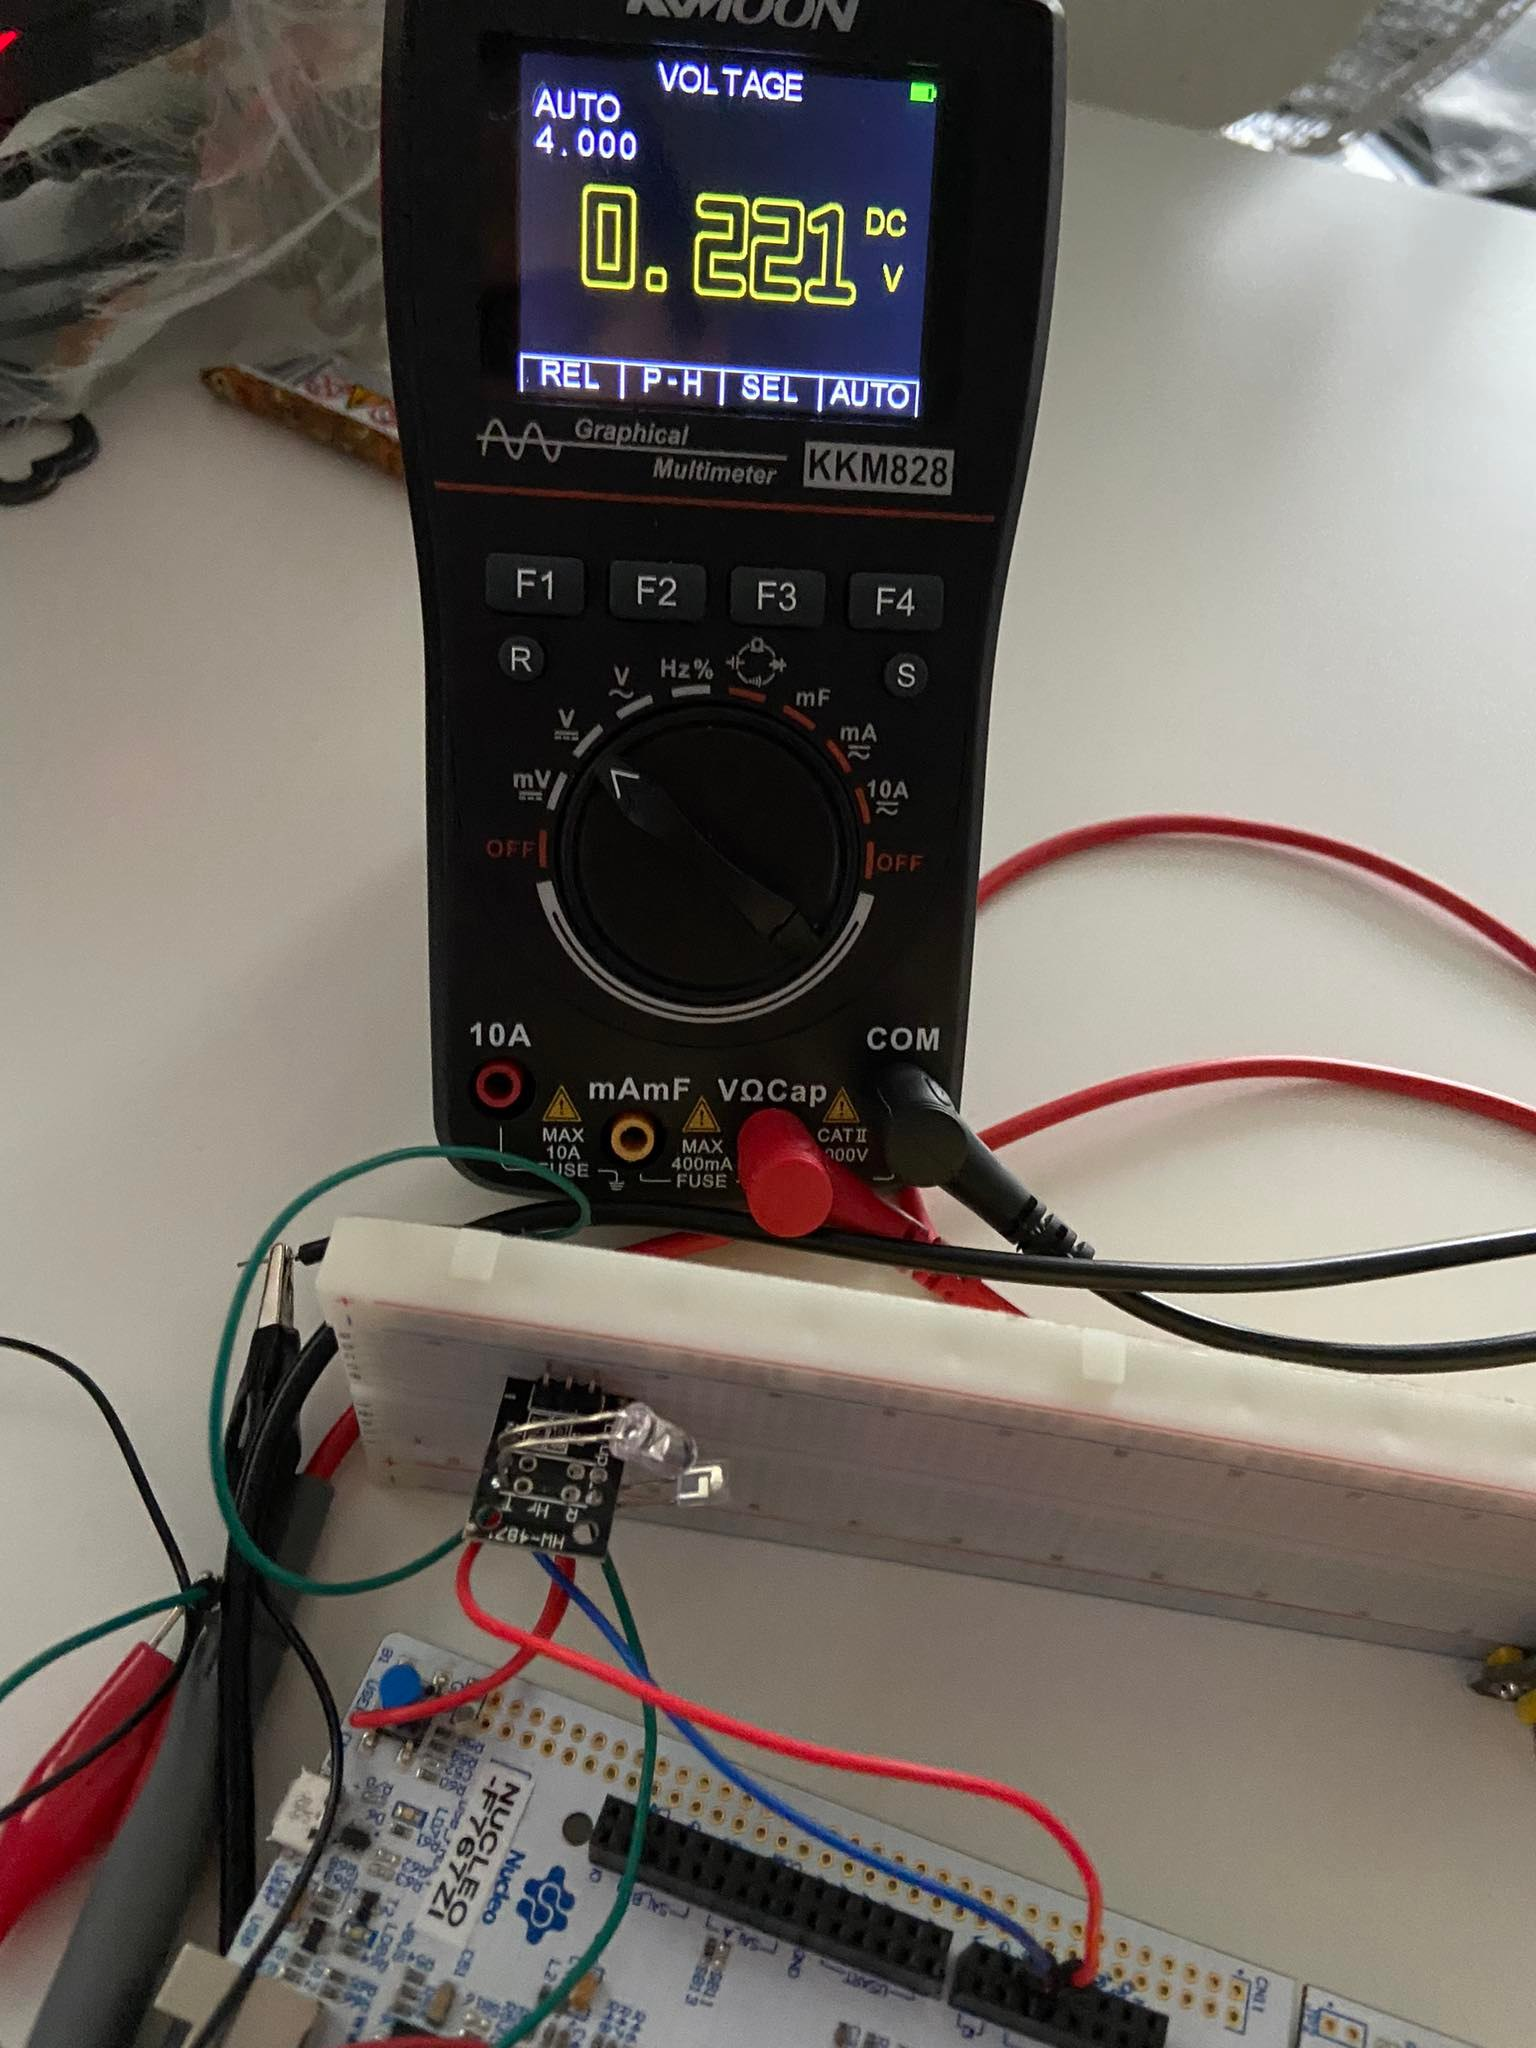
\includegraphics[width=.6\linewidth]{fig/KY-039/działanie_ukladu/bez_palca.jpg}
  \caption{Dużo światła dostaje się do fototranzystora}
  \label{fig:sub1}
\end{subfigure}%
\begin{subfigure}{.5\textwidth}
  \centering
    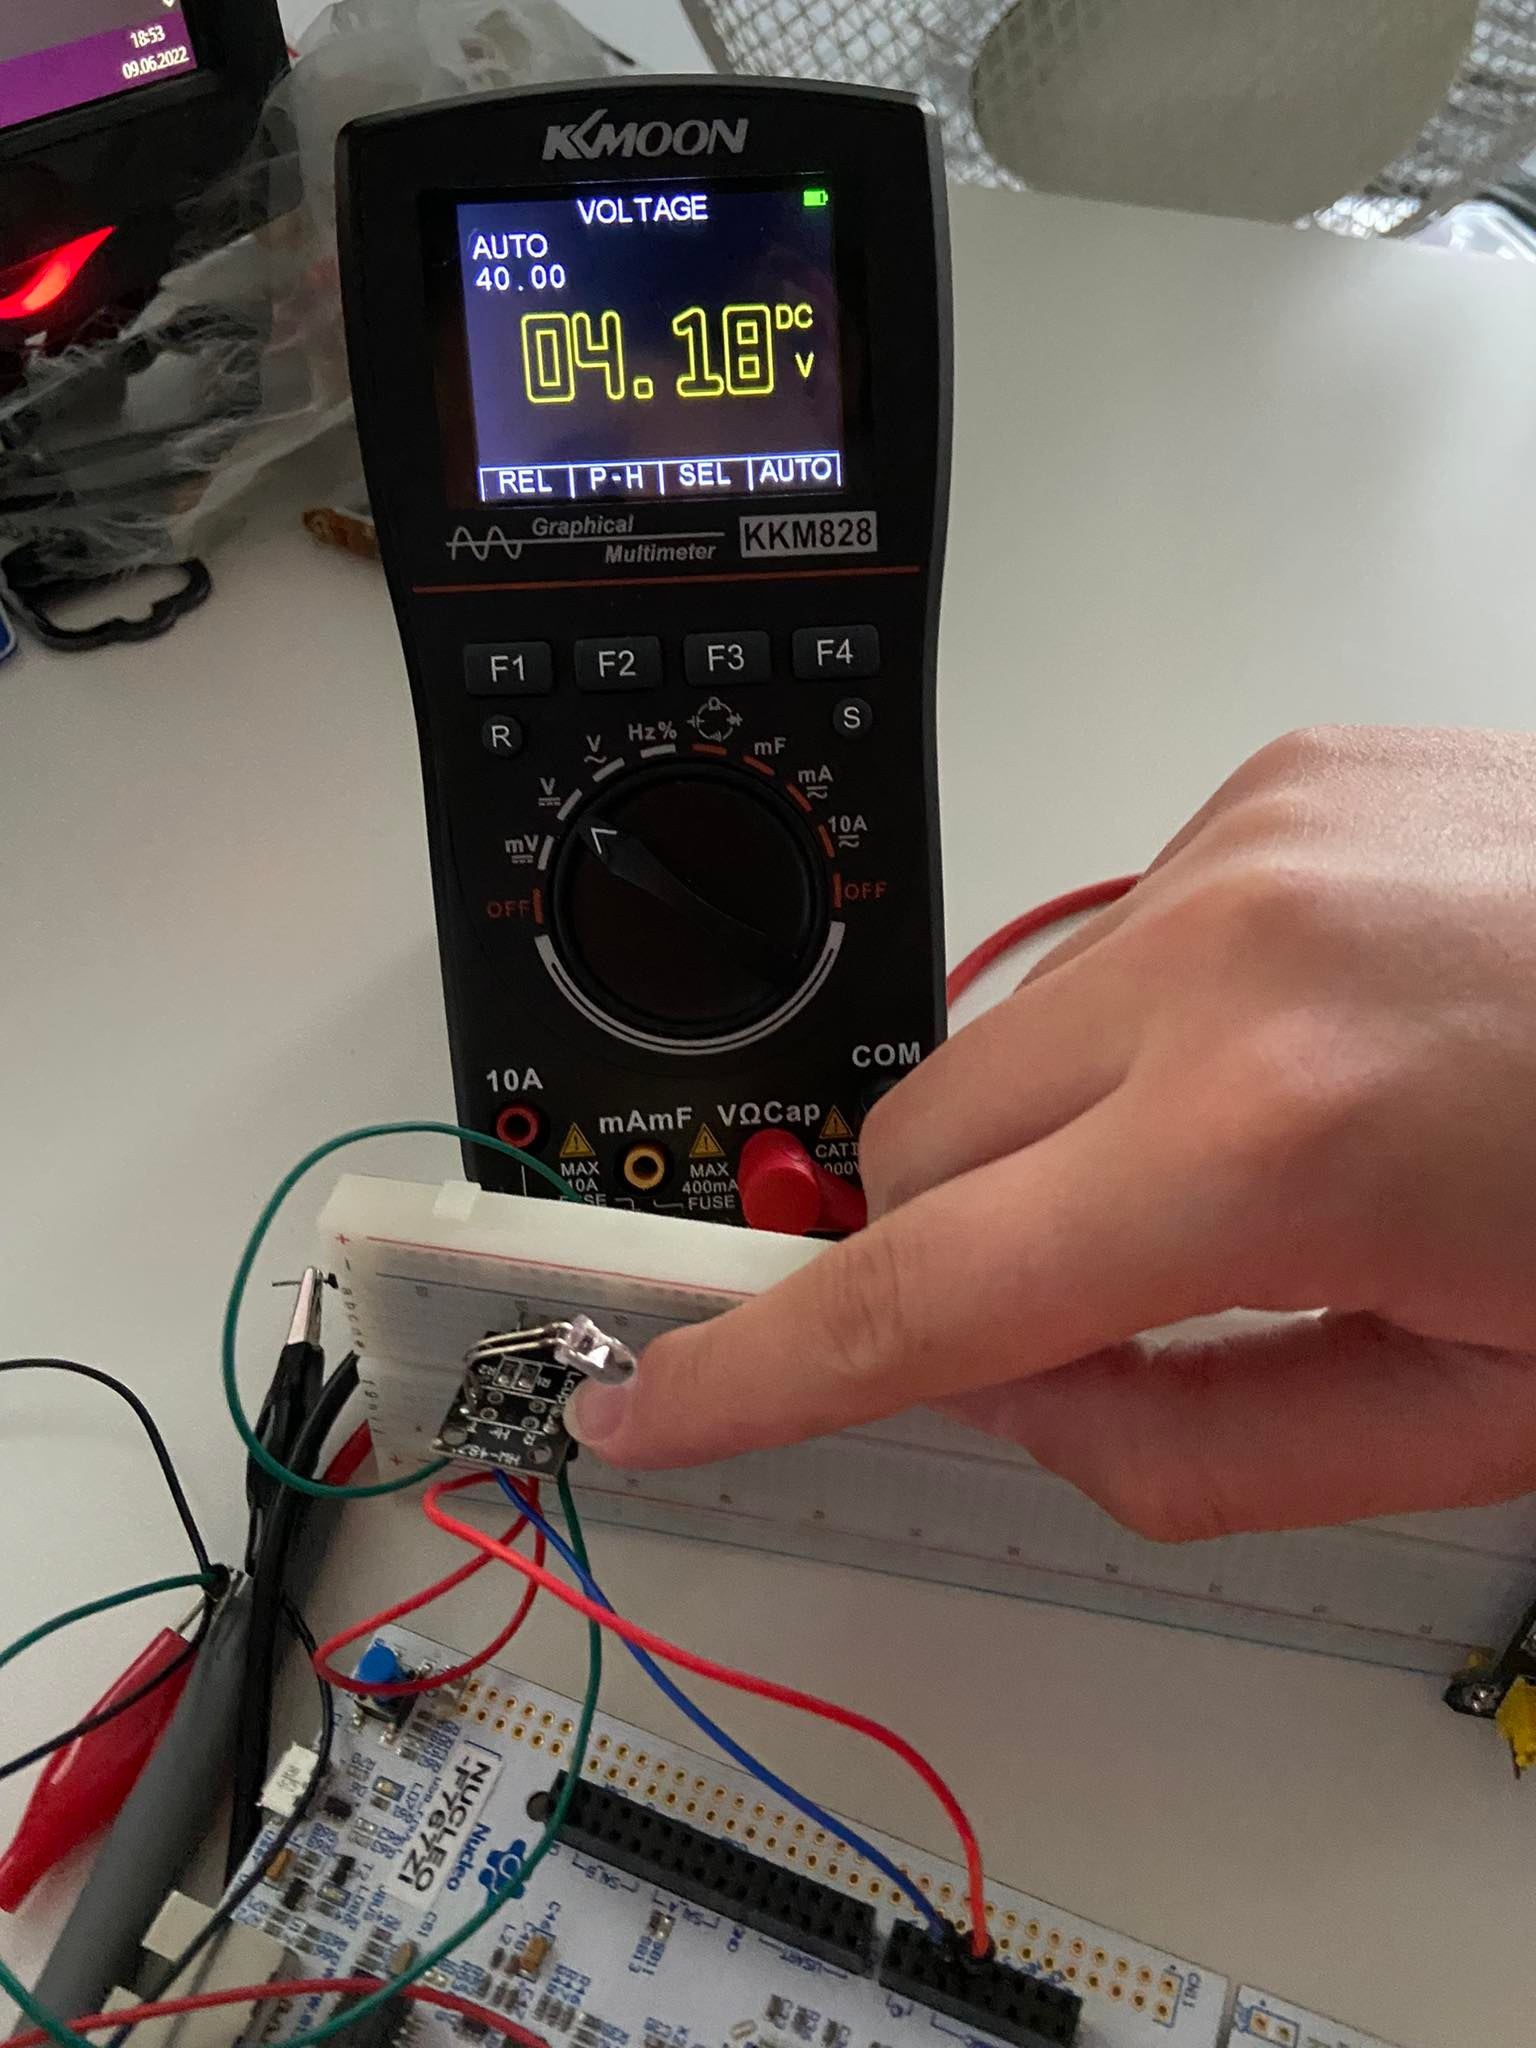
\includegraphics[width=.6\textwidth]{fig/KY-039/działanie_ukladu/z_palcem.jpg}
      \caption{Do fototranzystora dostaje się tylko światło przenikające przez palec. }
  \label{zd}
\end{subfigure}
\caption{Czujnik}
\label{fig:test}
\end{figure}
\vspace{0.5cm}

Czujnik jest bardzo wrażliwy na zakłócenia. Drobny ruch palcem powoduje zmianę amplitudy sygnału. Jest też możliwość, że w otoczeniu znajduje się inne niż dioda IR źródło światła podczerwonego, które będzie zakłócać odczyt.

\section{Prezentacja działania układu}
W celu zaprezentowania działania czujnika w układzie, połączono go do przetwornika ADC (pin PA\_3) w płytce NUCLEO-F767ZI oraz napięcia 3.3V. 

\begin{figure}[h]
    \centering
    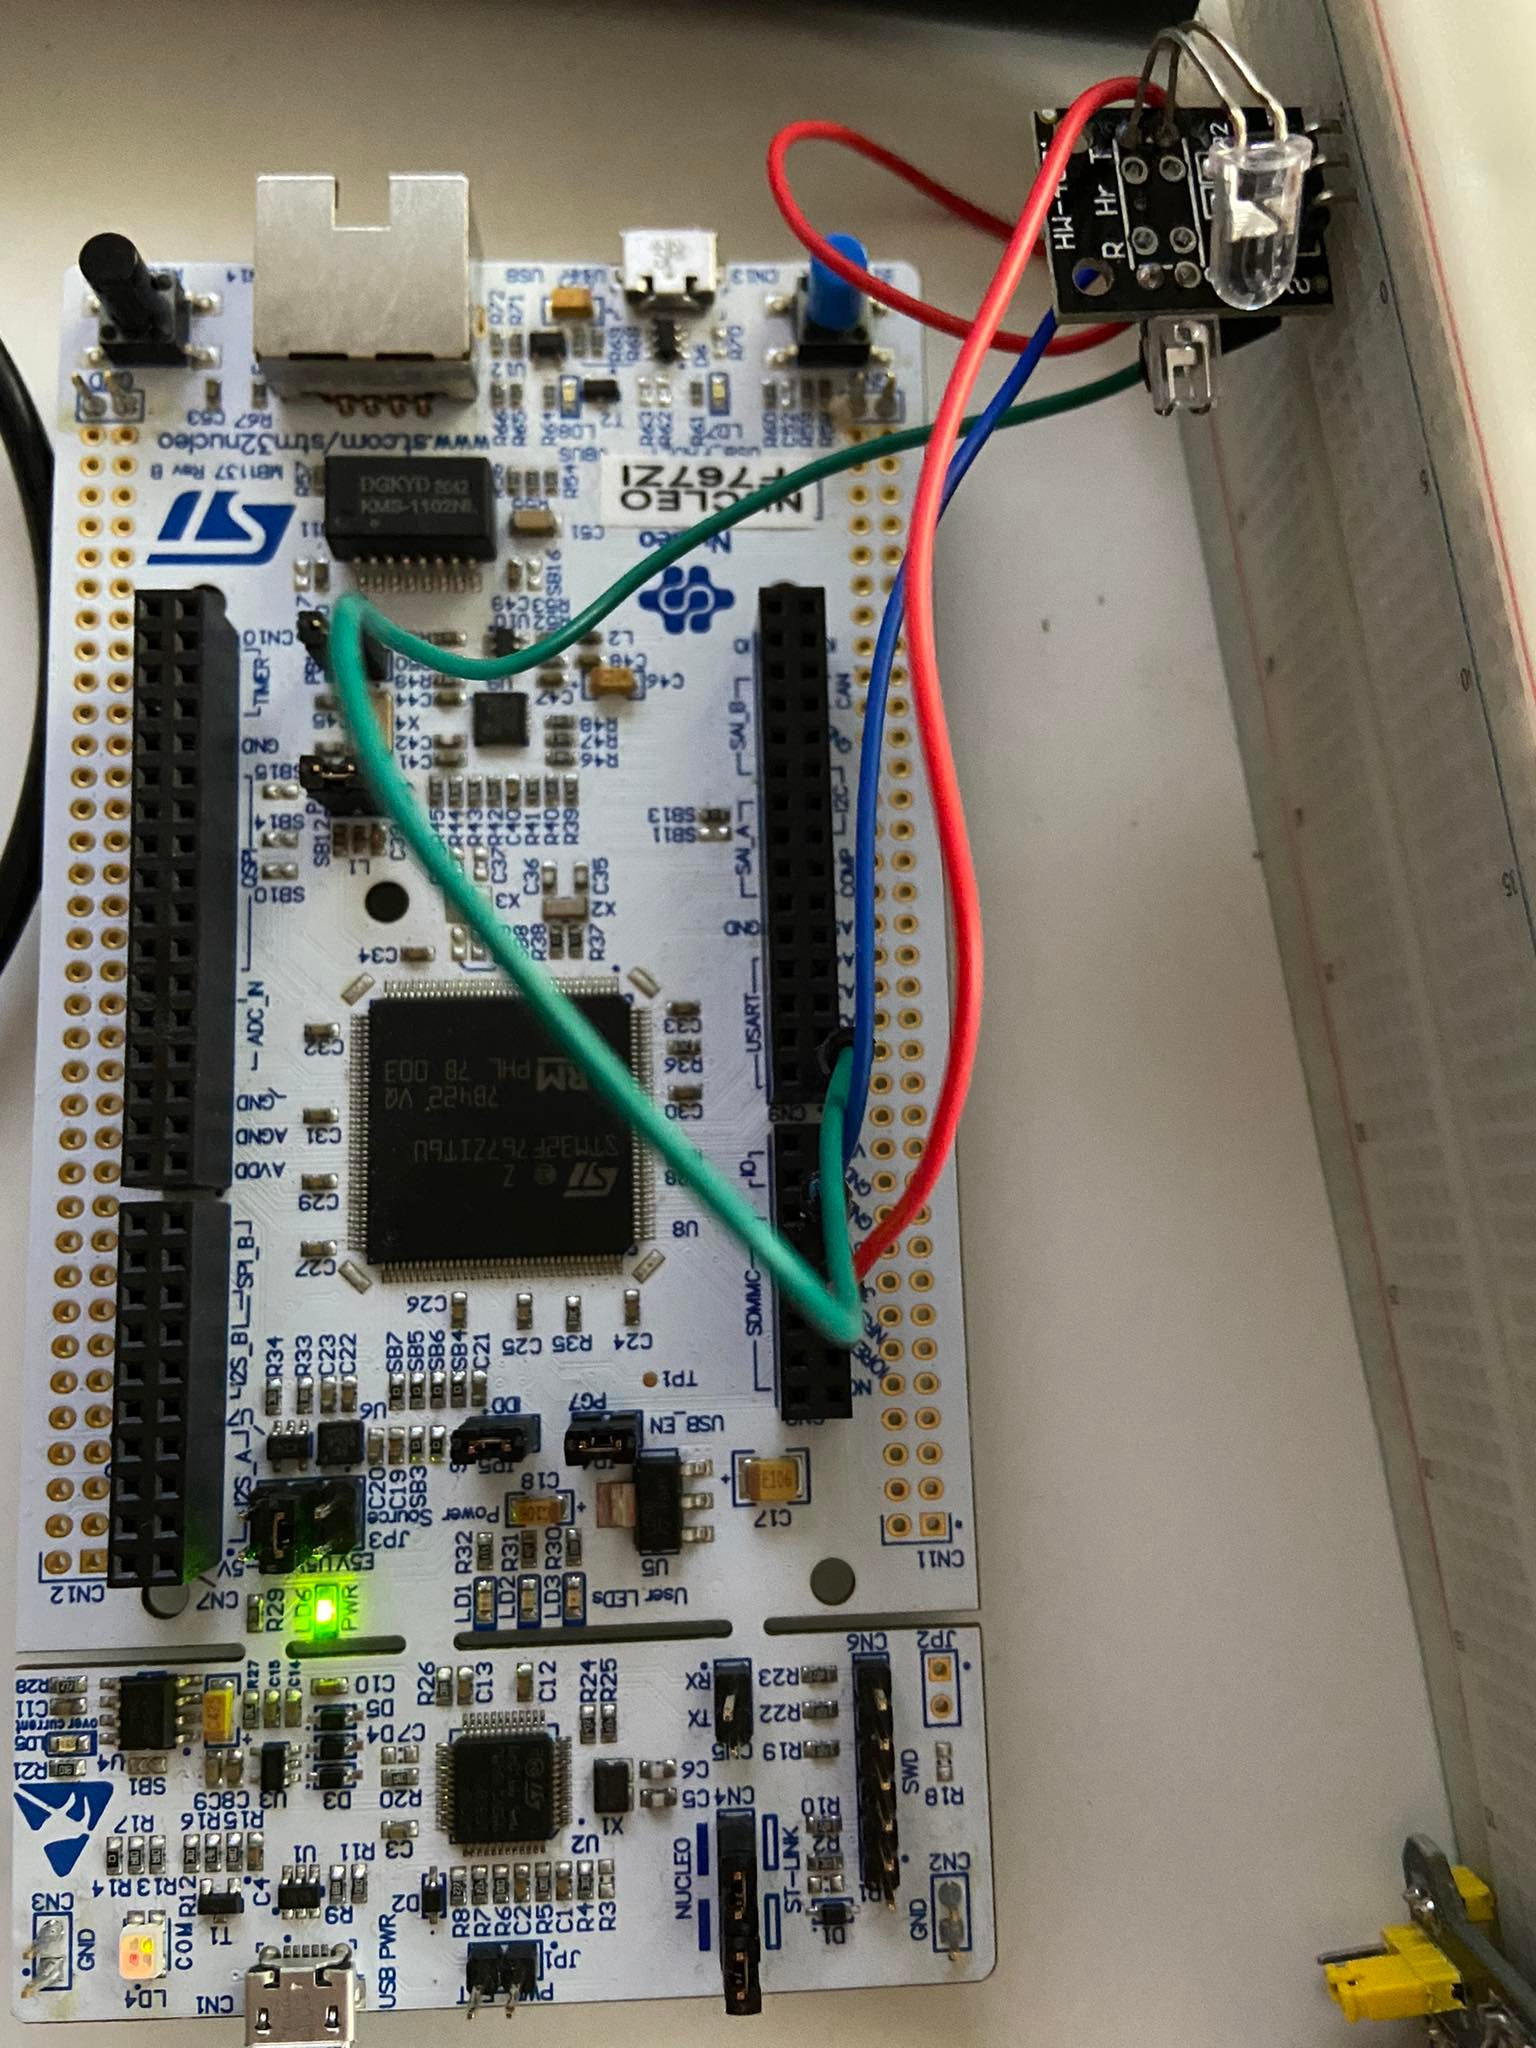
\includegraphics[width=0.6\textwidth]{fig/KY-039/działanie_ukladu/zdj3.jpg}
    \caption{Moduł podłączony do NUCLEO}
    \label{fig:my_label}
\end{figure}

\newpage
\vspace{0.5cm}
\begin{figure}[h]
  \centering
  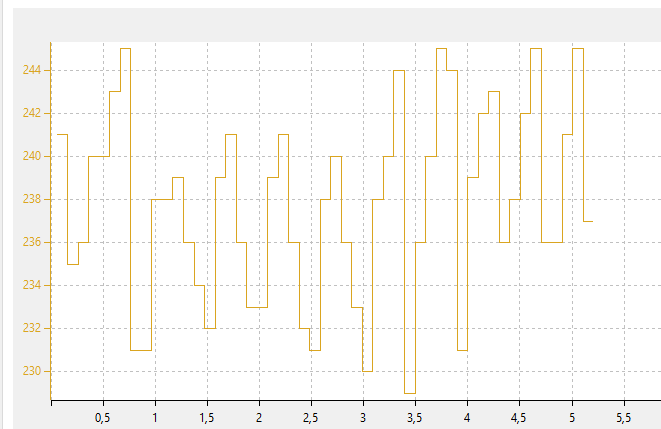
\includegraphics[width=.6\linewidth]{fig/KY-039/działanie_ukladu/adc_bezpalca.png}
  \caption{Bez palca}
\end{figure}
\begin{figure}[h]
  \centering
    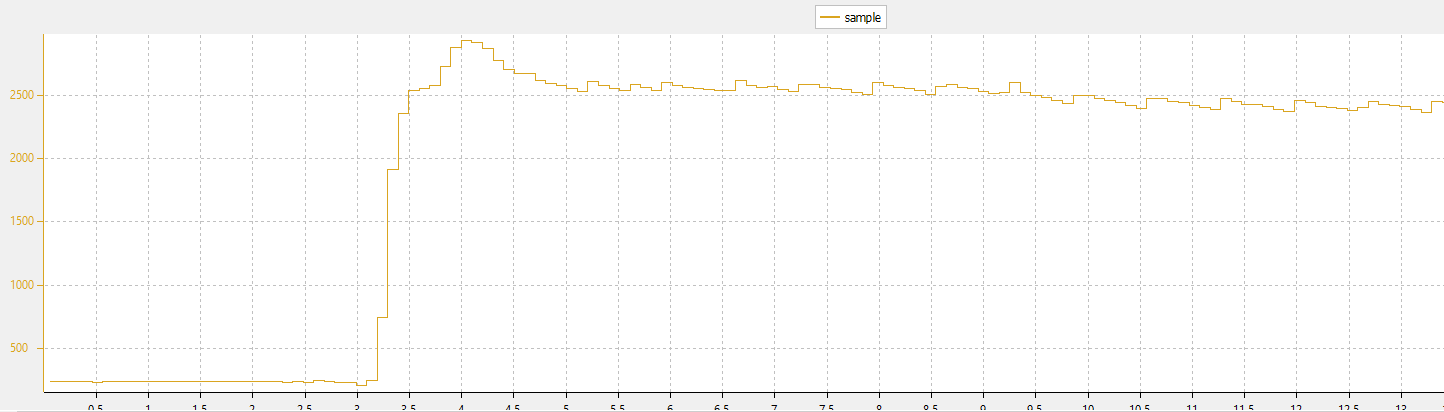
\includegraphics[width=.6\textwidth]{fig/KY-039/działanie_ukladu/adc_zpalcem.png}
      \caption{Po położeniu palca }
\end{figure}
\vspace{0.5cm}

Na drugim zdjęciu, po położeniu palca na fototranzystor widoczne są regularne wzniesienia i upadki w przebiegu, które reprezentują puls. 
\newpage
\printbibliography[heading=bibintoc]

\end{document}